\scanpage{107}
\margin{Cas critique \(N^{\frac{N-2}{2}},\ N^{\frac{N-1}{2}}\)
\figure{
\begin{tikzpicture}[x=.5cm,y=.5cm]\draw[line width=1.2pt](0,.3)--(0,0)--(1,0)--(1,.3);\end{tikzpicture}}}

\diagram{\begin{array}{ll}
A^i(X)\ \unsure{\text{---}|\longrightarrow}\ A^i(Y)&\text{bij si }i\leq\dfrac{N-3}{2}\\
&\text{inj. si }i\leq\dfrac{N-2}{2}
\end{array}}
\margin{Cas critiques \(i=\dfrac{N-2}{2},\ \dfrac{N-1}{2},\ \dfrac N2\)}

\margin{\unsure{conséquence} de 1° et 2°}
\textcircled{3}
\diagram{\begin{array}{ll}
A^i(X)\longrightarrow A^i(U)&\text{\uline{un isom} mod grp finis, }\forall i\\
&\text{\uline{un} \uline{isom} si }i\leq\dfrac{N-1}{2}
\end{array}}
\margin{[N.B. si \deleted{\(\unsure{i\geq N}\)} \(i\geq\dfrac{N+1}{2}\), \(A^i(X)\) et \(A^i(U)\) sont finis !]}
\diagram{\begin{array}{ll}
A^i(Y)\longrightarrow A^{i+1}(X)&\text{\uline{nul} \unsure{mod} grp finis, }\forall i\\
&\text{nul si }i\leq\dfrac{N-1}{2}
\end{array}}
\margin{[N.B. si \(i\geq\dfrac N2\), \(A^i(Y)\) est un grp fini !]}

\textcircled{4}\quad\uline{Pb}\quad Définir des formes ``\unsure{d'intersections|d'intersection}''
\[
N^i(X)\times N^i(X)\ \unsure{\longrightarrow|\text{---}}\ Z\ ??
\]
Définir pour \(J^{\unsure{\frac{N-1}{2}|\frac{N-2}{2}}}(X)\longrightarrow J^{\frac{N-1}{2}}(Y)\) resp. \(N^{\frac{N-2}{2}}(X)\longrightarrow N^{\frac{N-1}{2}}(Y)\) une théorie des cycles évanescents \(\text{------}\)
\figure{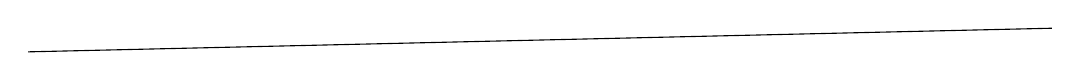
\begin{tikzpicture}\draw (0,0)--(13,.3);\end{tikzpicture}}

\uline{Ex}\quad \(N=2\)

\textcircled{1}\quad\(\boxed{N^1(X)\ \text{fini}}\) : c'est le th. \uline{de \deleted{\unsure{Lef}} Mumford-Hodge}.

\textcircled{2}\quad vide

\textcircled{3}\quad \deleted{\(\unsure{A^1(X)}\longrightarrow\)} vide

Groupe \(\unsure{+}\) essentiel \(J^1(X)\)
\margin{106}
